\subsection{{Maestría en sistemas embebidos}}
   \hypertarget{subsec:mse}
   En el marco de la MSE (Maestría en sistemas embebidos), se destacan los siguientes proyectos realizados: \\

   \cvlistitem{Python + sockets + threads + json + OOP}
      Para la asignatura \textit{Desarrollo de Aplicaciones sobre sistemas operativos de propósito general} se implemento un programa que utilizando Python, threads, sockets y bibliotecas de json, actualiza el cambio de moneda por UDP a un servicio remoto.
      Se puede consultar el código \faGithub\ en este \href{\linkgithubmsedaso}{link} y ver una demo siguiendo el link de la figura \ref{fig:mse_4_daso}
   \begin{figure}
      \begin{center}
         \href{\linkvideomsedaso}{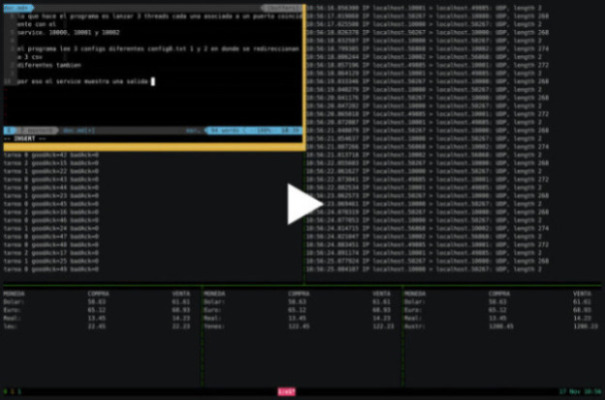
\includegraphics[width=0.6\textwidth]{mse_4_daso_asciinema.jpg}}
      \end{center}
      \caption{Desarrollo en Python con socket, threads, json y cvs en el marco de la maestría en sistemas embebidos.}
      \label{fig:mse_4_daso}
   \end{figure}
   \\
